\chapter{Resultados}
\label{cap:resultados}

\section{Alcance de los resultados}

Este capítulo informa identidades analíticas, comparaciones Monte Carlo sobre 13\,500 ejecuciones, una sensibilidad de ingeniería con 40\,500 trayectorias (sección~\ref{sec:engineering-sensitivity}) y una comparación reservada de mapas reducidos afines e híbridos sobre 9\,600 trayectorias (sección~\ref{sec:hybrid-results}). Todas las trayectorias provienen del micromundo especificado sin comisiones. La corrida reservada conserva el identificador \code{\RunID}; sus sumas de verificación y el comando de reproducción figuran en el anexo~\ref{cap:anexos}.

\section{Resultados analíticos: profundidad e impacto}
\label{sec:res-analitico}

Para una venta fija de $q=500$ unidades de $X$, el impacto $I(q,\kappa x)$ de la ecuación~\eqref{eq:impacto} crece al reducir la reserva (tabla~\ref{tab:impacto}). Con $x=10\,000$, reducir la reserva a la cuarta parte multiplica el impacto por 3.7 y el deslizamiento por 3.5.

\begin{table}[htbp]
\centering
\caption{Impacto de una venta de $q=500$ unidades según la reserva (resultado analítico).}
\label{tab:impacto}
\small
\begin{tabular}{@{}rrrr@{}}
\toprule
Factor de reserva & Reserva $x$ & Impacto $I$ & Deslizamiento (\%) \\
\midrule
1.00 & 10\,000 & 0.09758 & 4.76 \\
0.75 & 7500 & 0.12908 & 6.25 \\
0.50 & 5000 & 0.19062 & 9.09 \\
0.25 & 2500 & 0.36464 & 16.67 \\
\bottomrule
\end{tabular}
\end{table}

La figura~\ref{fig:impacto} muestra la curva completa. Con $I(q,\kappa x)=2\log(1+q/(\kappa x))$ y $\kappa<1$ se cumple $I(q,\kappa x)>I(q,x)$ para todo $q>0$, y la derivada de la ecuación~\eqref{eq:dI} es negativa. Este resultado es una consecuencia algebraica de la regla de producto constante y también sirve como control de la implementación (verificación 8 del anexo).

\subsection{Tasa ideal de corrección con arbitraje acotado}

En ausencia de otras órdenes y con referencia fija, un intercambio limitado a $q=cx$ cambia el precio logarítmico en una magnitud $\delta_c=2\log(1+c)$. Si el error está fuera de la banda, el exceso restante sigue $D_{t+1}=\max(0,D_t-\delta_c)$, y el número ideal de ticks hasta la banda es
\[
  N_\gamma=\left\lceil\frac{D_0}{2\log(1+c)}\right\rceil,\qquad D_0=(|e_0|-\gamma)_+.
\]
Para un choque logarítmico de magnitud $0.20$ y $\gamma=0.003$, se requieren idealmente 20 ticks con $c=0.005$, cuatro con $c=0.03$ y dos con $c=0.10$; con $c=0$ no hay corrección. Por tanto, el resultado de capacidad baja queda en gran medida implicado por la regla y el horizonte de 20 ticks. La simulación aporta información sobre cómo el ruido, la tendencia, el retiro y el orden de eventos alteran ese referente.

\begin{table}[htbp]
\centering
\caption{Corrección idealizada con referencia fija y sin otras órdenes.}
\label{tab:capacity-benchmark}
\small
\begin{tabular}{@{}rrr@{}}
\toprule
Capacidad $c$ & Corrección logarítmica por tick $2\log(1+c)$ & Ticks ideales hasta la banda \\
\midrule
0 & 0 & No hay corrección finita \\
0.005 & 0.00998 & 20 \\
0.03 & 0.05912 & 4 \\
0.10 & 0.19062 & 2 \\
\bottomrule
\end{tabular}
\end{table}

\begin{figure}[htbp]
\centering
\begin{tikzpicture}
\begin{axis}[width=0.78\textwidth,height=6cm,xlabel={Factor de reserva $\kappa$},ylabel={Impacto logarítmico $I$},grid=major,xmin=0.1,xmax=1.05]
\addplot[thick,blue!70!black] table[col sep=comma,x=reserve_factor,y=log_impact] {\datadir/impact_curve.csv};
\end{axis}
\end{tikzpicture}
\caption{Impacto logarítmico de una venta de $q=500$ unidades según el factor de reserva.}
\label{fig:impacto}
\end{figure}

\section{Panorama de las condiciones}

La tabla~\ref{tab:resumen} resume las cinco condiciones, con 2700 ejecuciones cada una (300 semillas por 9 celdas). E1-máx es una extrapolación fuera de los niveles principales de capacidad. Las 300 semillas son una decisión de réplica computacional, no el tamaño de una muestra de mercado.

\begin{table}[htbp]
\centering
\caption{Resumen de las condiciones reservadas (2700 ejecuciones por condición).}
\label{tab:resumen}
\small
\begin{tabular}{@{}lrrrrrr@{}}
\toprule
Condición & Área $A$ & $M$ legado & Recup. & Retorno\,$^{a}$ & Prof. mín. & Retiro \\
\midrule
E0 & 2.363 & 0.1012 & 4.6\,\% & 20.47 & 11667 & 0\,\% \\
E1-baja & 1.056 & 0.1305 & 56.8\,\% & 14.82 & 11667 & 0\,\% \\
E1-alta & 0.100 & 0.1220 & 100.0\,\% & 2.54 & 11667 & 0\,\% \\
E3 & 0.180 & 0.1335 & 96.6\,\% & 4.27 & 6417 & 100\,\% \\
E1-máx & 0.005 & 0.1197 & 100.0\,\% & 1.22 & 11667 & 0\,\% \\
\bottomrule
\multicolumn{7}{@{}l}{\footnotesize $^{a}$ Media restringida con censura en 21 ticks.}
\end{tabular}
\end{table}

El error pico medio es $0.176$ en E0, $0.127$ en E1-baja, $0.064$ en E1-alta, $0.073$ en E3 y $0.008$ en E1-máx. Ninguna orden estuvo limitada por capital en las 13\,500 ejecuciones.

\begin{figure}[htbp]
\centering
\begin{tikzpicture}
\begin{axis}[width=0.9\textwidth,height=6.4cm,xlabel={Tick},ylabel={$|d_t|$ medio},grid=major,legend pos=north east,legend style={font=\scriptsize},xmin=0,xmax=20,ymin=0]
\addplot[thick,red!70!black] table[col sep=comma,x=tick,y=mean_abs_excess,restrict expr to domain={\thisrow{series_id}}{10:10}] {\datadir/trajectories.csv};
\addplot[thick,orange!85!black] table[col sep=comma,x=tick,y=mean_abs_excess,restrict expr to domain={\thisrow{series_id}}{20:20}] {\datadir/trajectories.csv};
\addplot[thick,blue!70!black] table[col sep=comma,x=tick,y=mean_abs_excess,restrict expr to domain={\thisrow{series_id}}{30:30}] {\datadir/trajectories.csv};
\addplot[thick,dashed,green!50!black] table[col sep=comma,x=tick,y=mean_abs_excess,restrict expr to domain={\thisrow{series_id}}{40:40}] {\datadir/trajectories.csv};
\legend{E0,E1-baja,E1-alta,E3}
\end{axis}
\end{tikzpicture}
\caption{Exceso de error medio $|d_t|$ por tick, promediado sobre todas las celdas y semillas.}
\label{fig:trayectorias}
\end{figure}

\section{H1: corrección simulada frente al referente analítico}
\label{sec:res-h1}

El cálculo ideal predice 20 ticks hasta la banda con capacidad baja $c=0.005$, todo el horizonte de simulación; la regla de capacidad alta $c=0.03$ requiere solo cuatro ticks antes de que actúen los demás agentes. En las corridas reservadas, el área de exceso media es $2.363$ en E0, $1.056$ en E1-baja y $0.100$ en E1-alta. La diferencia pareada E1-alta menos E0 es $-2.263$ (mediana $-2.078$; intervalo bootstrap por semilla del 95\,\% $[-2.345,-2.182]$), y los promedios pareados de las 300 semillas son menores con E1-alta. La diferencia E1-alta menos E1-baja es $-0.956$ (intervalo $[-1.003,-0.909]$). Estos valores describen cómo el simulador especificado se aparta del referente simple; la dirección de la corrección por arbitraje se deriva de la propia regla.

\begin{table}[htbp]
\centering
\caption{Resúmenes Monte Carlo pareados (300 semillas). Los intervalos describen variación por semilla bajo el simulador fijo.}
\label{tab:inferencia}
\scriptsize
\setlength{\tabcolsep}{3pt}
\begin{tabularx}{\textwidth}{@{}>{\raggedright\arraybackslash}Xrr>{\raggedright\arraybackslash}p{0.25\textwidth}>{\raggedright\arraybackslash}p{0.16\textwidth}@{}}
\toprule
Contraste & Media $\Delta$ & Mediana & Intervalo 95\,\% & Signo \\
\midrule
H1: área E1-alta menos E0 & $-2.2629$ & $-2.0784$ & $[-2.3448,-2.1820]$ & 100\,\% menor \\
H1: área E1-alta menos E1-baja & $-0.9560$ & $-0.8456$ & $[-1.0034,-0.9091]$ & 100\,\% menor \\
H2: desplazamiento máximo legado & $+0.01143$ & $+0.01140$ & $[0.01074,0.01212]$ & 99.67\,\% mayor \\
H3 mapa menos persistencia, MAE & $-0.000808$ & $-0.000960$ & $[-0.000917,-0.000692]$ & 84.67\,\% menor \\
H3 mapa menos AR(1) escalar, MAE & $+0.0000822$ & $+0.0000844$ & $[0.0000780,0.0000864]$ & 97.67\,\% mayor \\
\bottomrule
\end{tabularx}
\end{table}

\subsection{Tasa de recuperación}

La recuperación sostenida depende de la capacidad y de la celda (tabla~\ref{tab:recuperacion}). Sin arbitraje apenas ocurre. Con capacidad baja varía entre 20 y 100\,\%, y es más baja cuanto mayor es el choque: un choque grande exige más pasos acotados por $c\,x$. Con capacidad alta y máxima es total en todas las celdas.

\begin{table}[htbp]
\centering
\caption{Tasa de recuperación sostenida (\%) por celda y condición.}
\label{tab:recuperacion}
\small
\begin{tabular}{@{}rrrrrrr@{}}
\toprule
$\kappa$ & Choque & E0 & E1-baja & E1-alta & E3 & E1-máx \\
\midrule
0.5 & $-0.05$ & 21.7 & 54.7 & 100.0 & 87.0 & 100.0 \\
0.5 & $-0.10$ & 1.3 & 45.3 & 100.0 & 86.7 & 100.0 \\
0.5 & $-0.20$ & 5.3 & 29.3 & 100.0 & 95.7 & 100.0 \\
1 & $-0.05$ & 0.0 & 72.0 & 100.0 & 100.0 & 100.0 \\
1 & $-0.10$ & 3.7 & 59.3 & 100.0 & 100.0 & 100.0 \\
1 & $-0.20$ & 0.0 & 20.3 & 100.0 & 100.0 & 100.0 \\
2 & $-0.05$ & 9.7 & 100.0 & 100.0 & 100.0 & 100.0 \\
2 & $-0.10$ & 0.0 & 99.0 & 100.0 & 100.0 & 100.0 \\
2 & $-0.20$ & 0.0 & 31.0 & 100.0 & 100.0 & 100.0 \\
\bottomrule
\end{tabular}
\end{table}

\subsection{Desglose por celda}

El efecto de H1 es negativo en todas las celdas (tabla~\ref{tab:celdas}); su magnitud crece con el choque, porque sin arbitraje el exceso se acumula durante los 20 ticks. La heterogeneidad entre semillas es grande (figura~\ref{fig:cuantiles}): el contraste va de $-4.60$ a $-1.38$.

\begin{table}[htbp]
\centering
\caption{Diferencia media por celda de los contrastes H1 (primario y de capacidad) y H2.}
\label{tab:celdas}
\small
\begin{tabular}{@{}rrrrrc@{}}
\toprule
$\kappa$ & Choque & E1-alta vs. E0 & E1-alta vs. E1-baja & Diferencia en $M$ legado & Reservada \\
\midrule
0.5 & $-0.05$ & $-1.630$ & $-0.832$ & $+0.0523$ & sí \\
0.5 & $-0.10$ & $-1.873$ & $-0.941$ & $+0.0361$ & sí \\
0.5 & $-0.20$ & $-3.128$ & $-1.703$ & $+0.0146$ & sí \\
1 & $-0.05$ & $-1.222$ & $-0.294$ & $0.0000$ & sí \\
1 & $-0.10$ & $-2.023$ & $-0.652$ & $0.0000$ & no \\
1 & $-0.20$ & $-3.784$ & $-1.883$ & $0.0000$ & sí \\
2 & $-0.05$ & $-1.007$ & $-0.116$ & $0.0000$ & sí \\
2 & $-0.10$ & $-1.951$ & $-0.450$ & $0.0000$ & sí \\
2 & $-0.20$ & $-3.748$ & $-1.732$ & $0.0000$ & sí \\
\bottomrule
\end{tabular}
\end{table}

\begin{figure}[htbp]
\centering
\begin{tikzpicture}
\begin{axis}[width=0.8\textwidth,height=6cm,xlabel={Cuantil},ylabel={Contraste por semilla},grid=major,legend pos=south east,legend style={font=\scriptsize}]
\addplot[thick,blue!70!black,mark=*,mark size=1.5pt] table[col sep=comma,x=quantile,y=value,restrict expr to domain={\thisrow{contrast_id}}{1:1}] {\datadir/delta_quantiles.csv};
\addplot[thick,orange!85!black,mark=square*,mark size=1.5pt] table[col sep=comma,x=quantile,y=value,restrict expr to domain={\thisrow{contrast_id}}{2:2}] {\datadir/delta_quantiles.csv};
\legend{H1 primario,H1 capacidad}
\end{axis}
\end{tikzpicture}
\caption{Cuantiles del contraste por semilla de H1 ($\Delta_1$ y comparación de capacidades).}
\label{fig:cuantiles}
\end{figure}

\section{H2: sensibilidad al retiro y a la escala de las órdenes}
\label{sec:res-h2}

Con el estadístico legado $M=\max_t|\log(p_t^D/p_0^D)|$, la diferencia pareada E3 menos E1-alta es $+0.0114$ en promedio (intervalo bootstrap por semilla del 95\,\% $[0.0107,0.0121]$). Este estadístico mide el desplazamiento respecto del precio del AMM previo al choque, no el sobrepaso ni el error máximo de seguimiento respecto de la nueva referencia CEX. Además, se satura en $|\text{choque}|+\gamma$ en seis de nueve celdas. Por tanto, el valor se conserva únicamente como descripción del diseño original.

Las diferencias por celda de la tabla~\ref{tab:celdas} son positivas solo con factor de profundidad $\kappa=0.5$ y nulas con $\kappa=1$ y $2$. El retiro se activa en todas las trayectorias E3 porque cada choque aplicado supera el umbral fijo $|e_t|>0.02$; normalmente ocurre en el tick 1. Esto es una intervención determinista única bajo los choques ensayados, no una prueba de adaptación heterogénea o gradual. La orden de pánico se activa solo con $\kappa=0.5$, donde el impacto configurado de la orden de ruido es 1.6\,\%, apenas 0.1 puntos porcentuales por encima del umbral de 1.5\,\%.

En la sensibilidad con semillas nuevas, la diferencia de baja profundidad se reduce al desactivar el pánico y desaparece en todas las profundidades cuando los tamaños de orden escalan con las reservas iniciales. La interpretación también está limitada por un acoplamiento de la implementación: el retiro reduce las reservas y por tanto también el límite de arbitraje $c x$. El diseño actual no identifica por separado el efecto del retiro y el cambio correspondiente en la capacidad de arbitraje. H2 es así una sensibilidad exploratoria de una regla, convención de órdenes y métrica particulares; no sustenta una afirmación general de amplificación de liquidez.

Un experimento rediseñado debería variar los umbrales entre proveedores, usar el error de seguimiento poschoque y el sobrepaso direccional como resultados distintos, variar la escala orden/reserva y mantener la capacidad de arbitraje independiente de las reservas. Esta tesis no incluye resultados de ese diseño.

\section{H3: comparación predictiva con referencias simples}
\label{sec:res-h3}

El mapa de dos estados se ajusta al exceso de error con signo $d_t$, que vale cero dentro de la banda y cambia de pendiente en su límite. Una sola relación afín no puede representar exactamente este umbral. En celdas reservadas, el mapa tiene menor error absoluto medio que la persistencia en la mayoría de condiciones, pero no supera al AR(1) escalar en ninguna condición principal. Por tanto, su segundo estado no demuestra valor predictivo incremental a un paso en este diseño; el mapa queda como resumen descriptivo del simulador, no como modelo de regímenes.

\begin{table}[htbp]
\centering
\caption{Error absoluto medio a un paso en celdas reservadas del simulador.}
\label{tab:h3}
\small
\begin{tabular}{@{}lrrrc@{}}
\toprule
Condición & Mapa dos estados & Persistencia & AR(1) escalar & Mapa mejora persistencia \\
\midrule
E0 & 0.01765 & 0.01751 & 0.01757 & no \\
E1-baja & 0.01573 & 0.01615 & 0.01566 & sí \\
E1-alta & 0.00493 & 0.00620 & 0.00486 & sí \\
E3 & 0.00929 & 0.01096 & 0.00916 & sí \\
E1-máx$^{\ast}$ & 0.00567 & 0.00594 & 0.00578 & sí \\
\bottomrule
\multicolumn{5}{@{}l}{\footnotesize $^{\ast}$ Condición de extrapolación fuera de los niveles principales de capacidad.}
\end{tabular}
\end{table}

Promediada sobre las cuatro condiciones principales, la diferencia mapa menos persistencia es $-0.000808$ (intervalo bootstrap por semilla del 95\,\% $[-0.000917,-0.000692]$); la diferencia mapa menos AR escalar es $+0.0000822$ (intervalo $[0.0000780,0.0000864]$). Estos intervalos describen variación Monte Carlo. Las etiquetas de trayectorias finitas resumen las mismas corridas y no son regímenes observados de forma independiente. Una comprobación anterior de Schur/Lyapunov ubicó todos los ajustes autónomos dentro del círculo unitario, incluido E0 con radio espectral 0.9978; no clasifica las trayectorias de horizonte finito.

\section{Comparación reservada de mapas afines e híbridos}
\label{sec:hybrid-results}

La nueva comparación usa el análisis 0.1.0, ejecución \code{\HybridRunID} y el error de precio con signo. En 9\,600 trayectorias reservadas de 300 semillas nuevas, el mapa híbrido redujo el MAE recursivo medio del error de precio de 0.030807 a 0.030291. La mejora pareada media fue 0.000516 (intervalo bootstrap por semilla del 95\,\% [0.000499, 0.000533]); el 99.7\,\% de los contrastes promediados por semilla favoreció a Hyb. La mejora media frente a L0 es de aproximadamente 1.7\,\%. Es una pequeña ganancia en error de reproducción dentro del simulador especificado; la evaluación recibe la trayectoria futura realizada del CEX y no constituye un pronóstico en tiempo real.

Cada condición aportó 12\,000 transiciones de selección. Hubo observaciones a ambos lados de la banda (tabla~\ref{tab:hybrid-regimes}), aunque el modelo de arbitraje bajo tuvo menos observaciones dentro de ella. El ajuste sigue siendo específico para cada condición, y estos conteos no demuestran que las dos variables de estado capturen toda la memoria relevante para la transición.

\begin{table}[htbp]
\centering
\caption{Transiciones de selección dentro y fuera de la banda configurada.}
\label{tab:hybrid-regimes}
\small
\begin{tabular}{@{}lrrr@{}}
\toprule
Condición & En banda & Fuera de banda & Total \\
\midrule
E0 & 681 & 11\,319 & 12\,000 \\
E1-baja & 1\,466 & 10\,534 & 12\,000 \\
E1-alta & 3\,776 & 8\,224 & 12\,000 \\
E3 & 2\,834 & 9\,166 & 12\,000 \\
\bottomrule
\end{tabular}
\end{table}

La mejora no se distribuye entre las condiciones operativas. Se concentra en el arbitraje de capacidad baja, especialmente con profundidad 2, donde la ganancia promediada entre los cuatro choques reservados es 0.003943. Con profundidad 0.5, la ganancia correspondiente es 0.000354. Los promedios de las demás combinaciones de condición y profundidad se encuentran entre aproximadamente $-0.000101$ y $-0.000002$, lo que favorece levemente a L0. El MAE secundario a un paso para $e$ mejora de 0.014882 a 0.014800, mientras que los errores a un paso y recursivos de la presión de flujo $z$ son ligeramente peores con Hyb. Por tanto, el resultado respalda una ventaja limitada y dependiente de la condición de los términos de banda para predecir el error de precio; no muestra una superioridad uniforme del mapa híbrido ni que las variables de estado representen todo el proceso.

\begin{figure}[H]
\centering
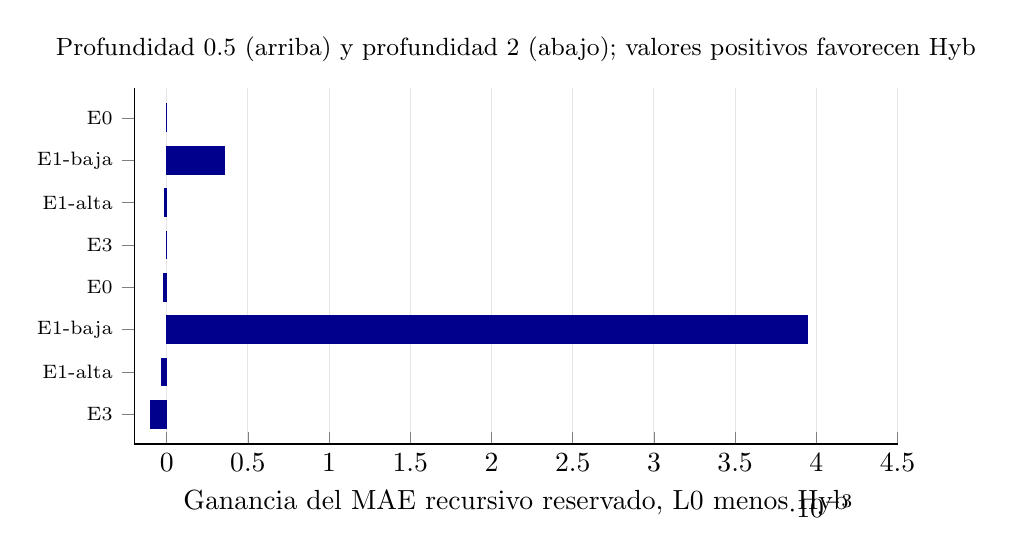
\begin{tikzpicture}
\begin{axis}[
  xbar, width=0.93\textwidth, height=6.1cm,
  xmin=-0.0002, xmax=0.0045,
  xlabel={Ganancia del MAE recursivo reservado, L0 menos Hyb},
  symbolic y coords={C1,C2,C3,C4,C5,C6,C7,C8}, ytick=data,
  yticklabels={E0, E1-baja, E1-alta, E3, E0, E1-baja, E1-alta, E3},
  yticklabel style={font=\scriptsize},
  y dir=reverse, xmajorgrids=true, grid style={gray!20},
  axis x line*=bottom, axis y line*=left,
  title style={font=\small}, title={Profundidad 0.5 (arriba) y profundidad 2 (abajo); valores positivos favorecen Hyb}
]
\addplot[fill=blue!55!black,draw=blue!55!black] coordinates {
  (-0.000002,C1) (0.000354,C2) (-0.000014,C3) (-0.000003,C4)
  (-0.000017,C5) (0.003943,C6) (-0.000033,C7) (-0.000101,C8)
};
\end{axis}
\end{tikzpicture}
\caption{Ganancia media del MAE recursivo del error de precio por condición operativa y profundidad. Cada barra promedia cuatro magnitudes de choque reservadas; los contrastes por celda son descriptivos y no tienen intervalos de confianza separados. Los valores se exportan en \code{figures/data/hybrid\_depth\_condition.csv}.}
\label{fig:hybrid-cell-gains}
\end{figure}

La ganancia media del mapa híbrido no debe interpretarse aisladamente: casi toda la ganancia proviene de una combinación de baja capacidad y profundidad, mientras que la predicción de la presión de flujo no mejora. El siguiente paso de modelado consiste en representar explícitamente los límites de capacidad y las transiciones de retiro de LP y evaluarlos con otro protocolo congelado, en vez de añadir más términos polinómicos libres. La comparación de mapas es un diagnóstico de reproducción dentro del simulador, no un pronóstico de mercado ni una afirmación de estabilidad del sistema completo.

\section{Trayectorias por profundidad}

La figura~\ref{fig:prof} compara E1-alta y E3 con $\kappa=0.5$. Con la menor profundidad, E3 parte del mismo exceso inicial y se corrige más despacio. Una explicación compatible es que el retiro reduce tanto la profundidad como el límite de arbitraje $c\,x$; estos mecanismos están acoplados en el diseño actual. Con $\kappa=1$ y $2$ las dos trayectorias son casi idénticas. El retorno sostenido ocurre en promedio en el tick $7.8$ para E3 con $\kappa=0.5$ frente a $2.8$ para E1-alta, mientras que con $\kappa=1$ y $2$ las diferencias son de $0.1$ ticks o menos.

\begin{figure}[htbp]
\centering
\begin{tikzpicture}
\begin{axis}[width=0.9\textwidth,height=6.2cm,xlabel={Tick},ylabel={$|d_t|$ medio},grid=major,legend style={font=\scriptsize},xmin=0,xmax=20,ymin=0]
\addplot[thick,blue!70!black] table[col sep=comma,x=tick,y=mean_abs_excess,restrict expr to domain={\thisrow{series_id}}{31:31}] {\datadir/trajectories.csv};
\addplot[thick,dashed,green!50!black] table[col sep=comma,x=tick,y=mean_abs_excess,restrict expr to domain={\thisrow{series_id}}{41:41}] {\datadir/trajectories.csv};
\legend{E1-alta,E3}
\end{axis}
\end{tikzpicture}
\caption{Exceso de error medio con $\kappa=0.5$: arbitraje alto estático (E1-alta) y con retiro adaptativo (E3).}
\label{fig:prof}
\end{figure}

\section{Sensibilidad de ingeniería: recuperación y escala de las órdenes}
\label{sec:engineering-sensitivity}

Un análisis suplementario (análisis 0.6.0, ejecución \code{\EngineeringRunID}) usó 300 semillas nuevas (2000--2299), tres variantes de flujo de órdenes y las 15 celdas de profundidad/choque/condición de la grilla de diseño reservada: 40\,500 trayectorias de 20 ticks abstractos. Es un análisis descriptivo y exploratorio de sensibilidad, no un contraste inferencial. La recuperación significa el primer par observado de ticks consecutivos dentro de la banda; las salidas posteriores se contabilizan por separado. Los plazos se expresan en ticks, no en tiempo transcurrido.

Con los tamaños absolutos originales, E3 adaptativo se recuperó al menos una vez en el 97.4\,\% de las trayectorias, pero solo el 81.9\,\% terminó dentro de la banda. De las trayectorias que se recuperaron, el 31.2\,\% salió después. Con profundidad 0.5, solo el 45.8\,\% terminó dentro de la banda y el 98.8\,\% de las trayectorias recuperadas salió posteriormente. Por tanto, en este modelo, un primer retorno sostenido no equivale a un seguimiento persistente. Estos promedios igualmente ponderados del diseño no sustentan una afirmación poblacional con ajuste por multiplicidad.

El contraste de respuesta máxima entre E3 adaptativo y estático cambia según la definición de las órdenes (tabla~\ref{tab:engineering-sensitivity}). Mantener fijos los tamaños absolutos produjo un efecto con profundidad 0.5; al escalar las órdenes de ruido y tendencia con las reservas iniciales, el contraste fue efectivamente cero en las tres profundidades. Desactivar la venta de pánico redujo el contraste de baja profundidad, pero no lo eliminó. Esto aísla un límite importante del modelo: la profundidad por sí sola no determina el resultado; también importan el tamaño de la orden relativo a las reservas y la regla de reacción.

\begin{table}[htbp]
\centering
\caption{Respuesta máxima suplementaria pareada: E3 adaptativo menos estático por profundidad (300 semillas nuevas). Intervalos aproximados del 95\,\% sin ajuste.}
\label{tab:engineering-sensitivity}
\small
\begin{tabular}{@{}lrrr@{}}
\toprule
Variante del flujo de órdenes & Profundidad 0.5 & Profundidad 1 & Profundidad 2 \\
\midrule
Órdenes absolutas fijas & 0.03458 [0.03225, 0.03690] & 0.00000 & 0.00000 \\
Órdenes proporcionales a reservas iniciales & 0.00000 & 0.00000 & 0.00000 \\
Órdenes fijas, sin pánico & 0.01471 [0.01364, 0.01577] & 0.00000 & 0.00000 \\
\bottomrule
\end{tabular}
\end{table}

Con profundidad 0.5 y órdenes absolutas fijas, E3 adaptativo terminó dentro de la banda en el 45.8\,\% de las trayectorias; con órdenes proporcionales, terminó dentro en el 100\,\%. Estas variantes comparten el mismo modelo estilizado de agentes representativos y no constituyen comparaciones empíricas. Los resúmenes por celda, contrastes pareados, configuración y hashes completos se exportan en \code{figures/engineering/}.

\section{Resumen de los resultados}

\begin{itemize}
  \item \textbf{Referente analítico del arbitraje:} una piscina aislada con capacidad $c$ reduce el error logarítmico fuera de la banda hasta en $2\log(1+c)$ por tick. Con $c=0.005$, el tiempo ideal de corrección para el choque grande ensayado ocupa todo el horizonte de 20 ticks; el signo del efecto de arbitraje activo se deriva de la regla especificada.
  \item \textbf{Sensibilidad al retiro:} el disparador actual se activa en todas las corridas de la condición adaptativa. El estadístico legado de desplazamiento desde el precio previo al choque es sensible a la profundidad y a la convención de tamaño de órdenes; su efecto de poca profundidad desaparece al escalar las órdenes con las reservas. No demuestra una amplificación general de liquidez.
  \item \textbf{Persistencia de la recuperación:} el 31.2\,\% de las trayectorias que volvió a la banda salió de ella después; con factor de profundidad $0.5$, la proporción fue 98.8\,\%. En este simulador, el primer retorno y el seguimiento sostenido son resultados distintos.
  \item \textbf{Modelos reducidos:} el mapa de dos estados mejora la persistencia en algunas condiciones, pero no supera al AR(1) escalar. La ganancia de cerca de 1.7\,\% del mapa sensible a la banda se concentra en una condición y utiliza la trayectoria futura realizada del CEX.
\end{itemize}
